\documentclass[twocolumn,preprintnumbers,amsmath,amssymb,superscriptaddress]{revtex4}
%\usepackage[pdftex]{graphicx}

\usepackage{amsmath,amsfonts,amssymb}
\usepackage[english]{babel}
\usepackage[latin1]{inputenc}
\usepackage[T1]{fontenc}
\usepackage{color}
\usepackage{float}
\usepackage{verbatim}
\usepackage{graphicx}
\usepackage{bm}
\usepackage{mathtools}
\usepackage{stmaryrd}
\usepackage{anyfontsize}


\graphicspath{{../Anime/figures/}}


%\usepackage{epstopdf}
%\usepackage{array}
%\usepackage{tabularx}
%\usepackage{multirow}
\usepackage{color}
%\usepackage{multibox}
%\usepackage{rotating}
%\usepackage{lineno}
%\usepackage[left]{lineno}
%\usepackage[comma,sort&compress]{natbib}
%\usepackage{authblk}
%\usepackage{multicol}

%\bibliographystyle{ieeetr}


%\linenumbers
%\setlength\linenumbersep{3pt}

\begin{document}



\author{Justin D. Yeakel} \affiliation{School of Natural Sciences, University
  of California, Merced, Merced, CA 95340, USA}

\author{Mathias Pires} \affiliation{}

\author{James O'Donnell} \affiliation{}

\author{Marcus de Aguiar} \affiliation{}

\author{Paulo Guimar\~aes Jr} \affiliation{}

\author{Dominique Gravel} \affiliation{}

\author{Thilo Gross} \affiliation{}

%\title{Simple rules yield complex communities: deconstructed species interactions and the assembly of communities}
%\title{Community assembly and dynamics by the deconstruction of species interactions}
\title{Quantization of ecological interactions yields insights into community assembly and dynamics}
%\author{Justin D. Yeakel${}^{1,2,*}$, Christopher P. Kempes${}^{2}$, \& Sidney Redner${}^{2,3}$ \\ \\
%${}^1$School of Natural Science, University of California Merced, Merced, CA \\
%${}^2$The Santa Fe Institute, Santa Fe, NM \\
%${}^3$Department of Physics, Boston University, Boston MA \\
%${}^*$To whom correspondence should be addressed: jdyeakel@gmail.com
%}


\begin{abstract}
abstract goes here
\end{abstract}

\maketitle

\section*{Introduction}

Amazing words. The best words.



\section*{Model Description}

%The scale of the model
% \textbf{The ANIMe Model} We examine assembly and dynamics of communities where we consider the interaction constraints determining colonization and extinction of species.
% The underlying dynamic that determines whether a species can colonize the community lies in the extent to which its various interactions with other species are satisfied.
% As such, the ANIMe model tracks the presence/absence of species over time, but does not incorporate changes in abundance.
% We assume that the abundance of all species in a given community are $>0$ and infer persistence based on the combination of interactions between species.
\textbf{The ANIMe Model} We aim to examine how interdependencies between species in communities either aid or inhibit both assembly and extinction over long timescales, and specifically how ecosystem engineers contribute to these dynamics.
We approach these questions by considering both multiple types of interactions between species -- including but not limited to trophic interactions --  as well as indirect interactions between species and `objects' that are introduced by the presence of ecosystem engineers.
Such introduced objects are to be considered in the abstract, and serve to represent either resources, habitat, or environmental alterations that are introduced by the engineers that make them, and can be utilized by others. 


\begin{figure}
\centering
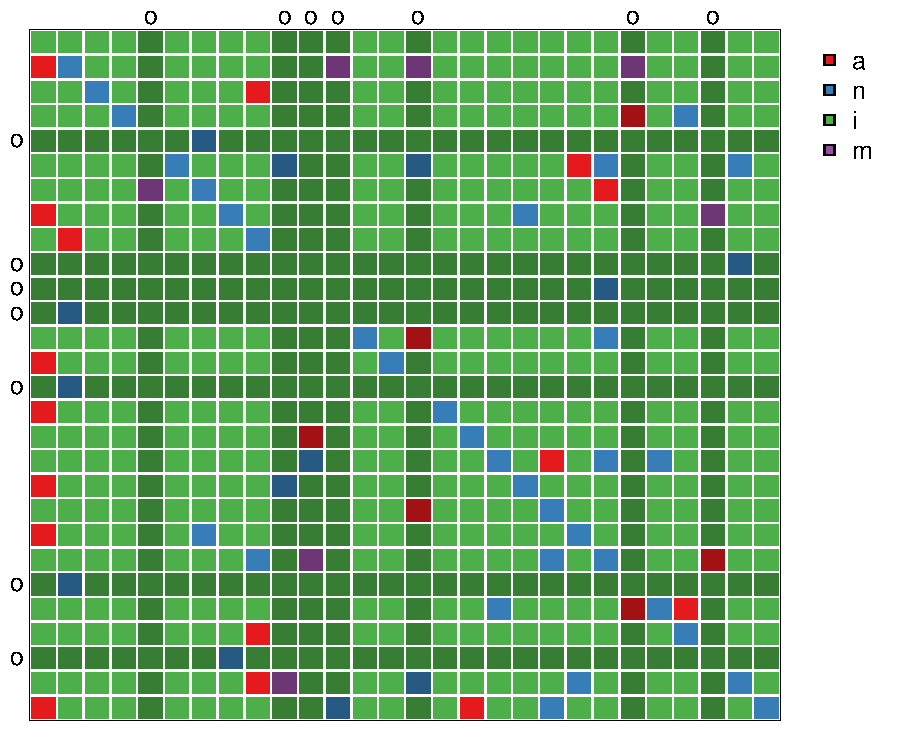
\includegraphics[width=0.45\textwidth]{matrix.pdf}
\caption{
An example of the source pool interaction matrix where $\mathcal{S} = 50$. Species and objects are aligned across the rows and columns; objects are shaded and labeled by `o' to distinguish them from species. The interaction recorded in row $i$ and column $j$ describes the directed interaction from species/object $i$ to species/object $j$. The first row/column represents the basal resource; species that assimilate the primary resource are capable of primary production. Species interact with other species and/or objects; objects only interact with their engineers by `needing' them; objects do not interact with other objects.
}
\label{fig:matrix}
\end{figure} 

%Interaction types

The ANIMe model consists of four directed interactions:
$a$: assimilate, which specifies a dependency involving biomass flow,
$n$: need, which specifies a dependency that does not involve biomass flow,
$i$: ignore, the null interaction, and
$m$: make, which connects a species to an object that it engineers. 
`Objects' are interactive components that can be made by $\geq 1$ species, and needed, assimilated, or ignored by the others.
We also note that such objects are to be considered in the abstract, as they could represent actual molecules or tissues that a species makes (e.g. oxygen respired by plants), habitat a species provides (e.g. as an elephant clears savannas of trees, facilitating shrubs), or even an abiotic condition (e.g. example). 

The four directed interaction types describe specific dependencies that one species/object has on another, however it is the coupling of two opposing directed interactions that describe traditional and familiar ecological relationships (listed in Table 1).
For example, an $a \leftrightarrow i$ interaction describes a typical predator-prey relationship, where species 1 assimilates species 2, and species 2 ignores species 1.
Of course, a prey's abundance does not \emph{ignore} predation, however our framework operates at the scale of presence-absence rather than abundance, and we assume that if both species are in the system, they have positive population densities, such that the state of the prey's occurrence effectively ignores the predator.
Both the $a \leftrightarrow n$ and $n \leftrightarrow n$ interactions describe service-resource and service-service mutualisms, respectively.
In the case of the former, one species interacts by way of a trophic interaction, whereas the other is provided a non-trophic need, such is the case in a plant-pollinator relationship.
Uniquely, the $m \leftrightarrow n$ interaction describes ecosystem engineering, where a species makes an object, while the presence of the object `needs' the presence of the species that makes it to exist.
Objects can be utilized by other species in the community, providing an indirect dependency that could be facilitated by multiple species (many engineers produce the same object) and/or used by multiple species (many species assimilate or need the same object).

We examine the assembly process of a novel community that emerges from a species pool.
The pool is a composite of species and objects that seeds the community, and may be imagined to be multiple pools that needn't be capable of coexisting.
In the following sections we will describe
1) how we build the species and their interactions within the source pool,
2) the rules for species assembly, and 
3) the rules for species extinction.



\textbf{Building the source pool} The source pool is generated by first setting the number of species $\mathcal{S}$ and then calculating how many objects $\mathcal{O}$ will be generated, which is stochastic from one source pool to the next.
To estimate the total number of objects, we first set the mean number of objects expected per species, ${\rm E}\{\mathcal{O}_i\}=\lambda$.
For each species, a set number of objects is drawn from ${\rm Poiss}(\lambda)$, such that the expected proportion of species that are engineers (species that make objects such that $\mathcal{}_i > 0$) is $1-{\rm e}^{-\lambda}$. 
If each species makes unique objects, the number of possible objects is $\mathcal{O}_{\rm max} = \mathcal{S}\lambda$, however because multiple species can make the same object, $\mathcal{O} \leq \mathcal{O}_{\rm max}$.
To determine whether objects are uniquely made or made by multiple engineers, we assign objects by randomly drawing object IDs from the integers $[1:\mathcal{O}_{\rm max}]$ without replacement and independently for each engineer; unassigned objects are discarded.
The expected total number of objects is thus 
\begin{equation}
{\rm E}\{\mathcal{O}\} = \mathcal{S}\lambda\left(1 - \frac{1}{{\rm e}}\right).
\end{equation}
The $m \leftrightarrow n$ interactions are thus determined upfront, and the proportion of `make' interactions in the $\mathcal{S} + \mathcal{O} \times \mathcal{S} + \mathcal{O}$ interaction matrix is calculated as
\begin{equation}
{\rm E}\{p_m\} = \frac{\lambda}{S\left(1 + \lambda - \frac{\lambda}{e}\right)^2}.
\end{equation}
For a given species-object interaction, the species `makes' the object, and the object `needs' the species that makes it.



Additional interactions within the source pool matrix are generated by setting the interaction probabilities $p_a$ and $p_n$, where $p_m$ is calculated from above, and $p_i = 1 - p_a + p_n + p_m$. 
We can then calculate the probabilities of pairwise interactions between both species and objects as 
\begin{align}
  p_{ai} &= p_i(p_a/(p_a+p_n+p_i)) + p_a(p_i/(p_a+p_i+p_n)), \\ \nonumber
  p_{an} &= p_n(p_a/(p_a+p_n+p_i+p_m)) + p_a(p_n/(p_a+p_i+p_n)), \\ \nonumber
  p_{aa} &= p_a(p_a/(p_i+p_n+p_a)), \\ \nonumber
  p_{nn} &= p_n(p_n/(p_a+p_n+p_i+p_m)), \\ \nonumber
  p_{ni} &= p_n(p_i/(p_a+p_n+p_i+p_m)) + p_i(p_n/(p_a+p_n+p_i)), \\ \nonumber
  p_{mn} &= p_n(p_m/(p_a+p_n+p_i+p_m)) + p_m, \\ \nonumber
  p_{ii} &= p_i(p_i/(p_a+p_n+p_i)).\\ \nonumber
\end{align}
The directional interaction between species $i \rightarrow j$ is thus described by the element in the $i^{\rm th}$ row and $j^{\rm th}$ column of the interaction matrix.

We build the interaction matrix for the source pool (figure \ref{fig:matrix}) according to the following steps:
1) We impose the rule that row/column 1 of the pool interaction matrix is the basal resource from which primary producers derive their energy.
Thus, an assimilate interaction in column 1 means that the consumer is capable of primary production; conversely, it is assumed that the basal resource does not interact with any species/objects.
Moreover, we assume that a fixed proportion of `assimilate' interactions across agents that must be linked to the basal resource, such that a given proportion of agents are capable of primary production.
The basal resource is assumed to be always available, and cannot be removed during the assembly process.

2) We next assume that -- initially -- all agents in the system are species, and assign trophic interactions based on an exponential degree distribution \cite{Williams:2000wt}.
The degree distribution is based on the trophic connectance of the system (where only links involving assimilation are involved), which in this case is calculated as 
\begin{equation}
  C_{\rm trophic} = p_{ai}+p_{an}+p_{aa}.
\end{equation}
For large communities, the number of trophic interactions for a given species $i$ in the Niche Model ($d_i$) is proportional to the niche range $r_i$, where $d_i = r_i*\mathcal{N}$ given $r_i = X\eta_i$, where $X \sim {\rm Beta}(1,1/2C_{\rm trophic} - 1)$ and $\eta_i \sim {\rm Uniform}(0,1)$ \cite{Williams:2000wt}. %is uniform in [0,1].
Importantly, because we do not stipulate which species are connected according to where the range falls within a niche axis (as is the primary function of the Niche Model), we incorporate the trophic interaction degree distribution without imposing a structure of interactions.
Accordingly, the only input to the interaction matrix of the source pool include the expected number of objects per species $\lambda$, the probabilities $p_a$ and $p_n$, and the exponential nature of the trophic degree distribution.
Given the drawn number of trophic interactions for each species, pairwise interactions $a \leftrightarrow i$, $a \leftrightarrow n$, and $a \leftrightarrow a$ are assigned randomly given $p_{ai}$, $p_{an}$, and $p_{aa}$, respectively.
Non-trophic species interactions $n \leftrightarrow i$ and $n \leftrightarrow n$ interactions are also assigned randomly given the respective probabilites $p_{ni}$ and $p_{nn}$, leaving only interactions involving species and objects to be determined.


3) The following rules are thus observed for species-objects interactions:
Objects are not allowed to `make' other objects.
Species can interact with objects (they may make, assimilate, or need them), however objects do not interact with anything except to `need' the engineers that make them.
Multiple species can make the same object: for example, most plant species engineer $O_2$, which is then used by other species.

% Finally, we declare that species with `make' interactions are engineers species that produce objects.
% Thus, a certain proportion of the agents in the system are declared species if there is a `make' interaction connecting them to another agent; the receiving agent is declared an object.
% When an object is declared, it ignores all other agents in the pool except for those species that make it (which are set to `need').
% Objects are not allowed to `make' other objects; if this occurs, the `m' interaction will be randomly assigned to a declared species.
% Species can interact with objects (they may make, assimilate, or need them), however objects do not interact with anything except to `need' the engineers that make them.
% Multiple species can make the same object: for example, most plant species engineer $O_2$, which is then used by other species.
% Because the number of `make' interactions is stochastic, the number of objects $\mathcal{O}$ and by extenstion the size of the pool $\mathcal{N} = \mathcal{S} + \mathcal{O}$ is also stochastic.
% To obtain the desired $\mathcal{S}$, we use a simulated annealing algorithm to generate multiple interaction matrices of different sizes until the desired $\mathcal{S}$ is found.



\textbf{Colonization and Extinction} The interaction matrix for the source pool specifies how each species interacts with every other.
Assembly of a species community is the result of both colonization and extinction of species that are drawn from the source pool.
The realized interactions within the assembled community are thus a subset of the potential interactions observed if every species were present.
However not all species can coexist in an assembled community at a given time.
We determine the colonization potential for a given species into a community as a function of two threshold conditions:
1) the colonizing species must assimilate at least one species/object, which may include the basal resource if that species is a primary producer, and
2) the colonizing species must satisfy a proportion of its need interactions, given by the threshold $n_t$; higher values of $n_t$ means that entry into the community is more difficult (a higher proportion of need interactions must be satisfied).
If the assimilate and need threshold conditions are both satisfied, colonization is permitted.
At each time-step $t$, we determine which species in the source pool can colonize the assembling community based on each meets the assimilate and need threshold conditions.
If multiple species can colonize, we select one at random and add it (and the objects it makes) to the community.
In the first time-step, only species that consume the primary resource (row 1; figure \ref{fig:matrix}) and do not have any `need' interactions can initiate the assembly process.

\begin{figure}
\centering
\includegraphics[width=0.4\textwidth]{predpreymotif.pdf}
\caption{
Non-specialist predators ($q=2$) consume a shared resource $i$, while each has alternative resources to fall-back on. Assuming Lotka-Volterra dynamics and equivalent attack rates of the predators $\beta$, the non-dimensional steady state density for the shared resource is $r_i^* = R_i^*/\kappa_i=1 - q\epsilon_i$ where $\epsilon_i=\beta P^*/\alpha_i$. We use this relationship between resource density and the number of predators $q$ to calculate extinction probabilities as a function of the number of predators $\omega_i(q)$
}
\label{fig:lv}
\end{figure} 


% The probability of extinction increasesas the number of consumers increases for a given species.
Although colonization depends only on satisfaction of assimilate/need interactions, persistence depends on
1) both assimilate and need thresholds remaining fulfilled, and
2) the pressure levied onto species by predation.
Although the ANIMe framework does not track population densities, we integrate a central concept from population dynamics: that resource densities decline with increased predation pressure, and that this increases the risk of extinction.
Assuming Lotka-Volterra predator-prey dynamics, a given resource $i$ has density $R_i$, growth rate $\alpha_i$, and carrying capacity $\kappa_i$.
The consumption of this resource by $q$ non-specialist predators with equivalent steady state densities $P^*$ and attack rates $\beta$ results in the dimensionless steady state resource density $r_i^* = R_i^*/\kappa_i = 1 - q\epsilon_i$, where $\epsilon_i=\beta P^*/\alpha_i$ (see figure \ref{fig:lv} for an exemplary motif illustrating the described interactions).
Thus, $\epsilon$ describes the relative impact of a single predator on the resource steady state, which decreases linearly with an increase in the number of predators $q$.
Although our framework does not track changes in population densities, if we assume that the true resource density is normally distributed around $r^*$ with variance $\sigma^2$, the probability of extinction $\omega_i$ (defined as the probability that $r^* < 0$) has an exact solution of the form
\begin{equation}
  \omega_i(q) = \frac{1}{2}{\rm Erfc}\left(\frac{1-q\epsilon_i}{\sigma\sqrt{2}}\right).
\end{equation}
The probability of extinction for a resource increases sigmoidally with the number of predators on that resource, and the number of predators where the probability of extinction is $\omega=0.5$ is given by $q(\omega=0.5) = 1/\epsilon$.
At each time-step, we calculate $\omega_i$ for each species in the assembled community and determine extinction by drawing from a binomial distribution where there is a single trial with success probability $\omega_i$.
Species that go extinct at time-step $t$ may re-colonize at $t+1$.
In this respect, each time-step is a colonization event and needn't be assumed to represent an equivalent length of time.

\begin{figure}
\centering
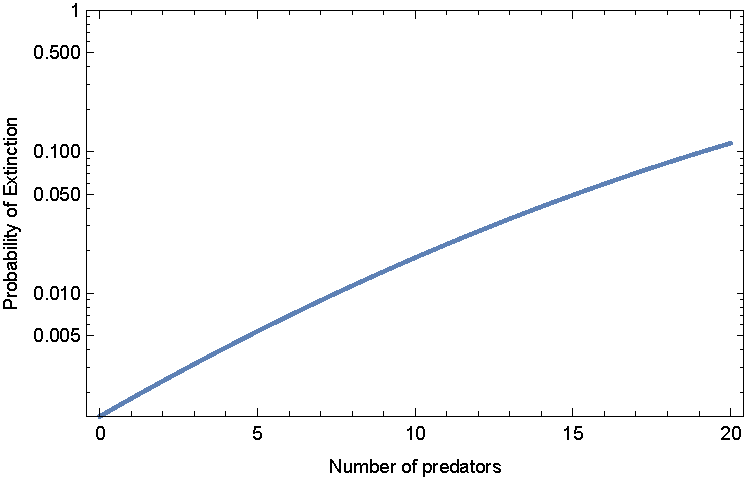
\includegraphics[width=0.45\textwidth]{extinction.pdf}
\caption{
The probability of extinction at time $t$ as a function of the number of predators consuming a given resource species $\omega_i(q)$. There is always \emph{some} risk of extinction even if a species has no predators, as $\omega_i(q=0) = 0.0014$.
}
\label{fig:ext}
\end{figure} 


Primary extinctions can trigger secondary extinctions, as elimination of prey -- and any objects that an eliminated species uniquely engineers -- may then result in consumers falling below either or both of the assimilate and need threshold conditions.
Accordingly, extinctions can cascade until the threshold conditions for every remaining species are satisfied.
We differentiate between extinctions that are initiated as the result of predation pressure (primary extinctions) from those that follow one or more primary extinctions (secondary extinctions).
Taken together, the community dynamics occur from a minimal set of rules:
\begin{enumerate}
  \item At time-step $t$, determine whether assimilate/need threshold conditions are met for each species in the source pool that isn't currently in the community
  \item Select at random a colonizing species and its attendant objects from this subset
  \item Assess the probability of extinction for all species in the assembling community
  \item Independently draw extinctions from a binomial distribution with a success probability equal to the extinction probabilities. Eliminate these species and any uniquely made objects from the community. These are \emph{primary extinctions}.
  \item Re-assess whether assimilate/need threshold conditions are satisfied in the post-extinction community. Eliminate those species and any uniquely made objects from the community that do not meet threshold conditions. If further extinctions occur, continue to re-assess threshold conditions until all species meet the requirements. Combined, these are \emph{secondary extinctions}.
  \item Time advances as t=t+1 and the process restarts.
\end{enumerate}
















% %Need discussion of 
% Ecological analogues: 
% As pr(n) increases, so does the number of mutualistic interactions (direct and indirect).
% As pr(m) increases, so does the number of engineers (and indirect interactions).
% As pr(a) increases, so does the connectance of trophic interactions (show how this is related).
% As $n_t$ increases, (this is the weird one), behavioral plasticity decreases in the sense that .
% 
% n-n: symbiont interaction

\begin{table*}[!t]
\begin{center}
\begin{tabular}{ l l l }
\hline
Parameter & Definition & Value/Range \\
\hline
$\overrightarrow{a}$ & assimilate & \\
$\overrightarrow{n}$ & need & \\
$\overrightarrow{i}$ & ignore & \\
$\overrightarrow{m}$ & make & \\
\hline
$a \leftrightarrow i$ & Asymmetric Predation &  \\
$a \leftrightarrow a$ & Symmetric predation & \\
$n \leftrightarrow a$ & Trophic mutualism & \\
$n \leftrightarrow n$ & Non-trophic mutualism & \\
$n \leftrightarrow i$ & Commensalism & \\
$i \leftrightarrow i$ & Null & \\
$m \leftrightarrow n$ & Engineering & \\
\hline
$\mathcal{N}$ & Number of species + objects & dyn.\\
$\mathcal{S}$ & Number of species & dyn.\\
$\mathcal{O}$ & Number of objects & dyn.\\
$a_t$ & Assimilate threshold & 0.0\\
$n_t$ & Need threshold & 0.2\\
$k$ & Number of consumers interacting with species $i$ & dyn.\\
$\omega_{\rm b}$ & Background probability of extinction at time $t$\\
$\omega(t)$ & Cumulative probability of extinction at time $t$ & $\frac{\omega_{\rm b} + \epsilon n}{1 + \epsilon n}$\\
$1/\epsilon$ & Number of consumers of resource $i$ at which $\omega_i(t)=\frac{1}{2}$ & 1000\\
\hline
\end{tabular}
\end{center}
\caption{Table of parameters, definitions, and assigned values or ranges.}
\end{table*}




\section*{Results \& Discussion}


% 
% 
% {\bf Community assembly without extinctions}
% In the context of community assembly, the niche space that is created by a given assemblage can be measured by evaluating the number of potential colonizers that can \emph{fit} within the assemblage from the species pool, fulfilling required assimilation and need threshold conditions.
% Because colonization without extinction does not account for resource limitation due to ever-expanding trophic loads of species that serve as resources for higher-trophic consumers, niche space is not reduced by packing more species into the community.
% However, because colonization from the mainland is a zero-sum event, with each successful colonization the number of potential future colonizers is reduced by one.
% Importantly, if a successful colonizer increases the number of potential future colonizers, this can be interpreted as functionally expanding the niche space of the community.
% 
% 
% 
% 
% Due to the competing effects of niche space expansion and species pool depletion, we find that the proportion of the species pool capable of successfully colonizing the assembling community is concave parabolic (Fig. \ref{fig_potcol}a).
% Early in the assembly process, the proportion of potential colonizers is equal to the proportion of species that are primary producers without an abundance of $n$ dependencies (too many need interactions precludes such primary producers from serving as initial colonizers).
% As assembly continues, niche space expands to a maximum, and then declines as the species pool diminishes and the community is filled.
% 
% 
% %Over pr(m)
% For a species pool of $400$, by changing the value of pr($m$) from 0.0001 to 0.002, we alter the proportion of engineers from ca. 0 to ca. 700.
% As the number of engineers is increased, the number of objects that they create -- and other species can interact with -- is likewise increased.
% For example, a single realization where $S=400$ species and pr(m)=$10^{-4}$ resulted in a $412\times412$ interaction matrix (400 species, 12 objects), while a realization with $S=400$ and pr(m)=$0.003$ resulted in a $1100\times1100$ interaction matrix (400 species, 700 objects).
% The former example generated a small number of engineers, each producing a single object, whereas the latter example generated a large number of engineers, each producing between 1-6 objects, with some objects being produced by multiple engineers.
% % 
% % \begin{figure*}[ht]
% % \centering
% % 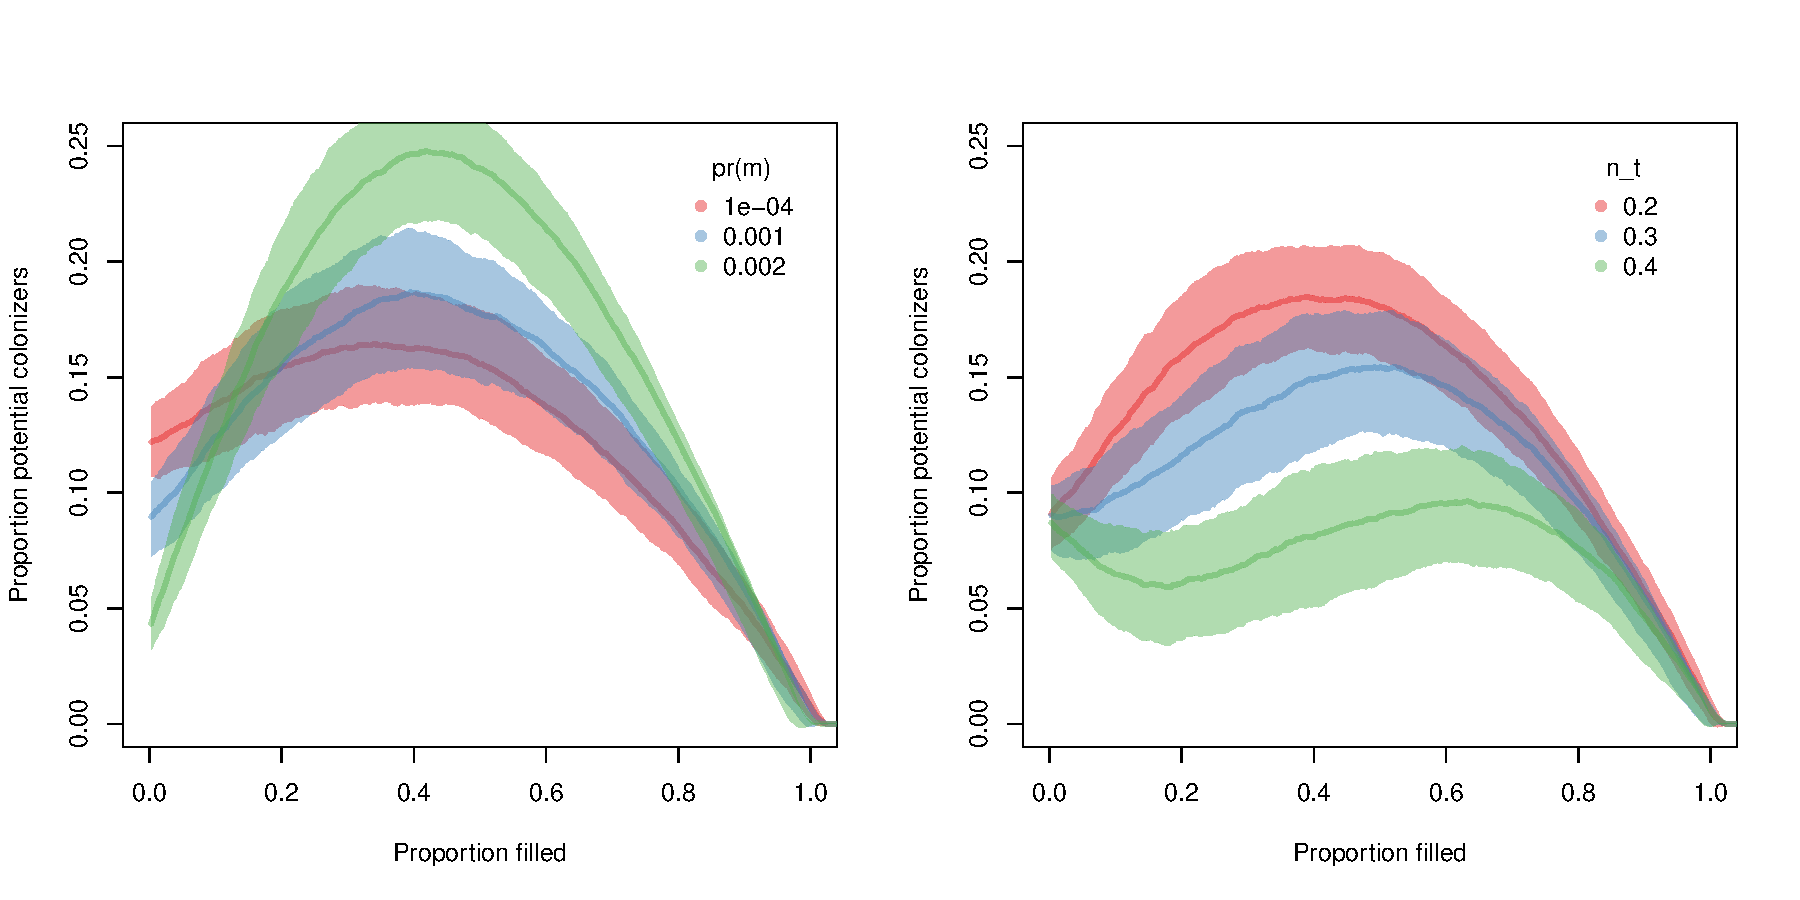
\includegraphics[width=0.9\textwidth]{fig_potcol_comb.pdf}
% % \caption{
% % a) Expansion of niche space (by counting the proportion of species that are capable of colonizing from the larger species pool) over systems with increasing number of engineers (increasing pr($m$)). b) Expansion of niche space over different need thresholds $n_t$. 
% % }
% % \label{fig_potcol}
% % \end{figure*} 
% 
% The effects of the proportion of engineers in the community on niche space expansion during assembly, and without the limiting forces of extinction, are substantial.
% While both limited-engineer and many-engineer systems resulted in a concave down niche expansion curve, the engineered system was different in three important ways.
% First, the many-engineer system began assembly with a smaller proportion of potential colonizers.
% This is due to the fact that there are many more interdependencies between species and objects, and as there are few objects carried over early in community development, the limitations on species are exaggerated.
% Second, the rate that niche space is expanded is higher for many-engineer communities
% Third, the production of objects by engineers nearly doubles the potential niche space (proportion of potential future colonizers) midway through assembly.
% Once there is a large enough base of colonizers in the assembling communities, there are enough objects present to facilitate rather than inhibit additional colonization opportunities.
% Thus, the influence of engineers during assembly - by creating more interdependencies between species and the objects they engineer - both constrains and promotes assembly at different stages of the process.
% 
% 
% %Over need_threshold
% Every species must satisfy at least one assimilate interaction, i.e. it must eat at least one other present species or basal resource.
% Moreover, every species must fulfill a certain proportion of its `need' interactions, set by the threshold parameter $n_t$.
% As $n_t$ increases, the interdependencies between species become more rigid during the assembly process, and this will serve to limit niche expansion.
% 
% However, the trajectory of niche expansion is more complex when $n_t$ is increased.
% Rather than simply lowering the proportion of potential colonizers, increasing $n_t$ results in a qualitatively different assembly process where niche space is first lowered, increased, and lowered again as the community is filled (Fig. \ref{fig_potcol}b).
% The initial niche space contraction results from a filling of the initial community with primary producers and their direct consumers.
% This lower trophic module fills without creating additional space for higher trophic level organisms due to the harsher restrictions given by a high $n_t$.
% Once a critical point in assembly is reached, the potential to add higher trophic level colonizers is attained, and niche space increases to a maximum, only to finally decrease as the species pool is used up.
% In some realizations, the community is never able to fill, resulting in a system without higher trophic levels.
% 
% Assembly where $n_t$ is large, and with moderate engineering, follows a 2-stage process.
% First, the system is colonized by primary producers.
% Once the lower trophic levels are filled and reach a critical point, niche expansion permits the colonization of higher trophic level colonizers.
% [Need to explore this more by calculating trophic level for each species - in progress]
% 
% 
% 
% 
% %Is there a diversity-stability link here?
% 
% 
% %Initial downward slope occurs because primary producers are used up. When it goes back up, there is enough of a base to build a larger community. Will have to check this will average trophic level over time (trophic module!!!)
% 
% 
% 
% 
% 
% {\bf Assembly with extinctions}
% % Negative effects of engineering at the scale of the community
% % The effect of engineers on extinction cascade size
% Examination of the assembly process that is regulated by extinctions due to changes in trophic load results in saturation of species richness over time (Fig. \ref{fig_traj}).
% Accordingly, the colonization and extinction dynamic result in regular fluctuations around a steady state community richness, where the size of the fluctuations (relative to the steady state value) strongly depends on $n_t$ and pr($(a,n$).
% 
% The average diversity of the system after an initial assembly process increases as the number of need interactions and/or need threshold $n_t$ are sufficiently low.
% This is intuitive because such a system has many more degrees of freedom and is free to expand to higher densities of species.
% Likewise, as pr($n$) and $n_t$ increase, species richness lowers nearly to zero, as does the average trophic level (check), resulting in a system dominated by primary producers and their immediate consumers.
% 
% 
% The system conforms to an expected Taylor's law relationship for lower species richness (<100), however follow different rules for higher richness (also corresponding to low pr($n$) and $n_t$.
% Here, species dependencies are low, such that primary extinctions due to predation will generally not result in a large number of secondary extinctions because the need threshold is not easily violated, and this reduces the magnitude of fluctuations.
% Accordingly, it is the same drivers that lead to high species richness (increased plasticity and/or fewer non-trophic dependencies) that also reduces the volatility of the system, thereby reducing variability.
% 
% 
% The magnitude of oscillations around the steady state richness is a measure of community instability and turnover.
% Although modification of pr($n$) and $n_t$ reveals a smooth and expected influence on the mean species richness of the community, the effect on the magnitude of fluctuations around the mean richness is more complex, and this is most evident in the coefficient of variation of community richness over time.
% The CV is maximized when $n_t$ is intermediate and the number of non-trophic dependencies is large.
% 
% % 
% % \begin{figure}
% % \centering
% % 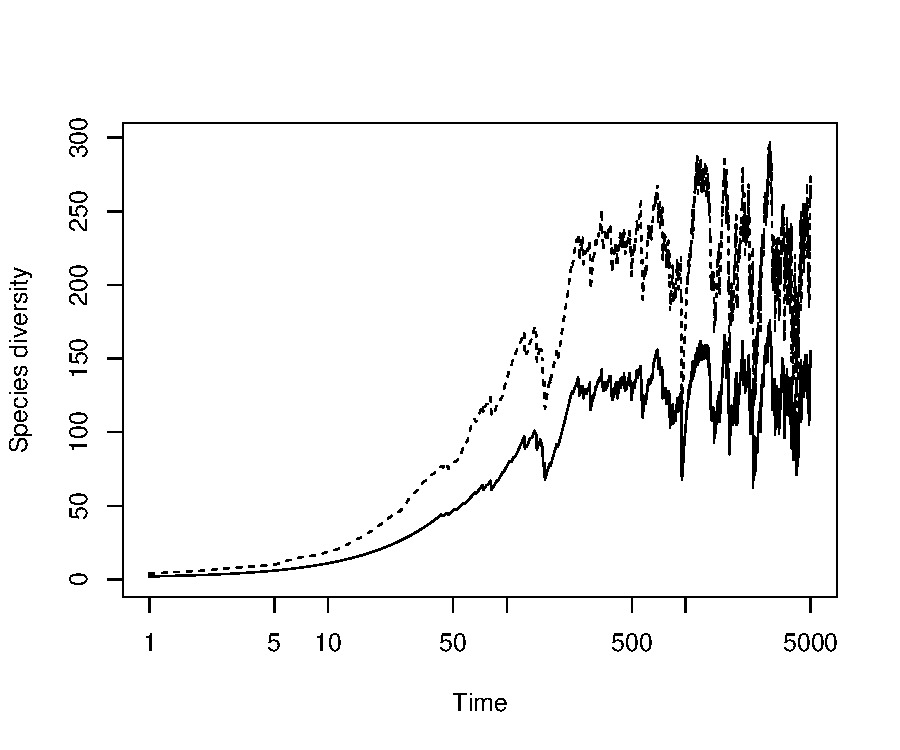
\includegraphics[width=0.45\textwidth]{fig_traj.pdf}
% % \caption{
% % The colonization and extinction dynamics of a community over time. The solid line denotes species richness; the dashed line denotes species+object richness.
% % }
% % \label{fig_traj}
% % \end{figure} 
% % 
% 
% 
% 
% {\bf Effects of engineers on community dynamics}
% We find that an increase in the number of engineers at time $t$ results in the potential for marginally larger extinction cascades at time $t+1$ (positive but weak correlations, Fig \ref{fig_corrobext}a).
% This weak positive correlation between the number of objects at time $t$ and extinction cascade size at time $t+1$ is due to the increasing interconnectedness that results from the higher number of objects relative to species in the system.
% Because the existence of a given object is tied to the species that makes them (one or multiple), the effects of primary extinctions are magnified.
% 
% % 
% % \begin{figure}
% % \centering
% % 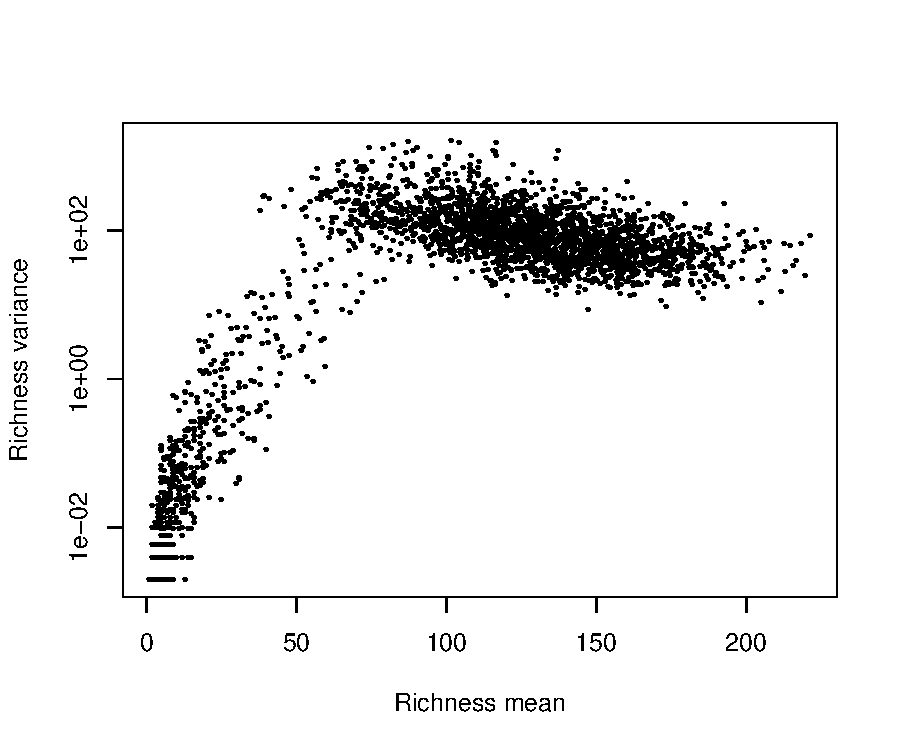
\includegraphics[width=0.45\textwidth]{fig_taylors.pdf}
% % \caption{
% % Relationship between mean species richness and the magnitude of fluctuations (SD) for communities with various values of pr($n$) and $n_t$.
% % }
% % \label{fig_traj}
% % \end{figure} 
% % 
% % 
% % \begin{figure}
% % \centering
% % 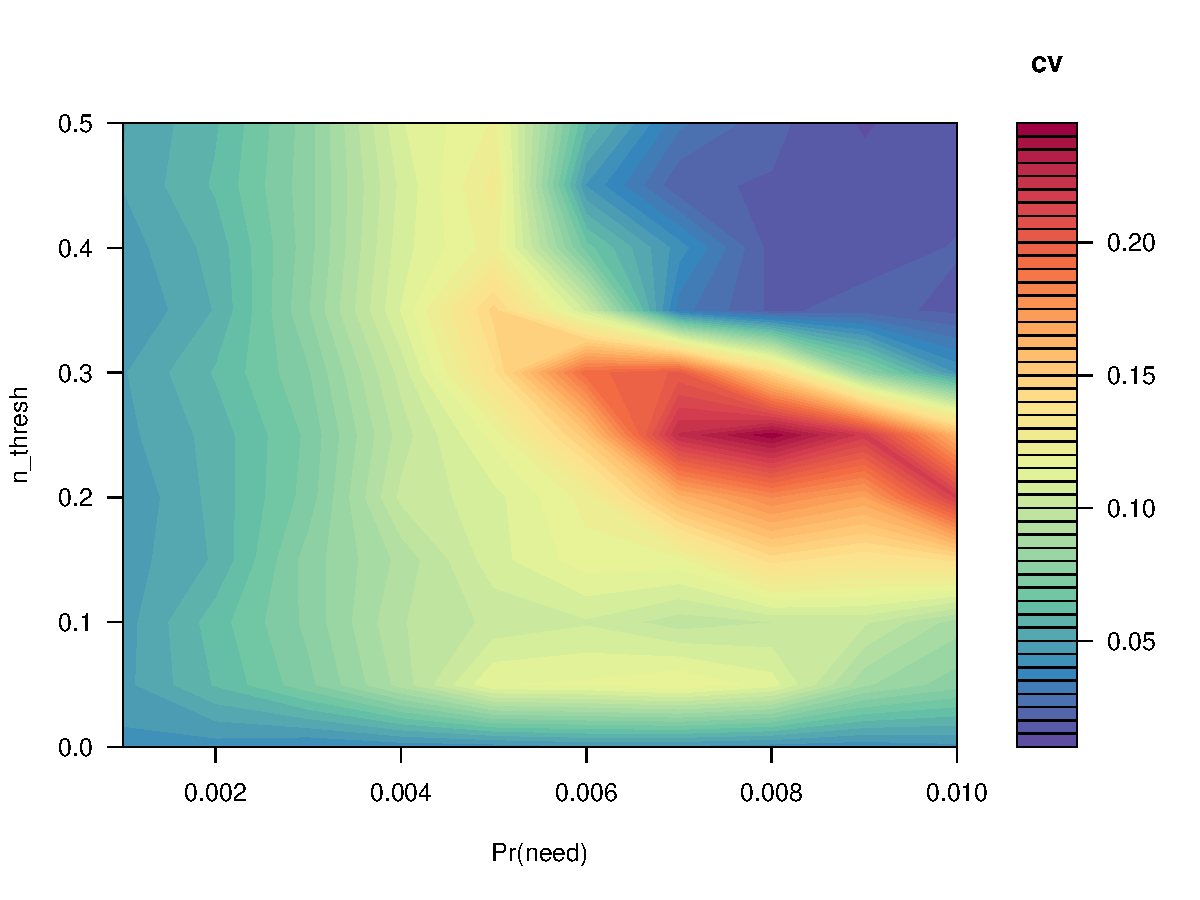
\includegraphics[width=0.45\textwidth]{fig_sen_nn.pdf}
% % \caption{Changes in community richness CV as a function of pr($n$) and $n_t$. 
% % }
% % \label{fig_sen_nn}
% % \end{figure} 
% % 
% 
% 
% 
% % The effect of engineering colonization facilitation
% The number of objects in the system at time $t$ (and by extension the number of engineers) is strongly positively correlated with the number of potential colonizers at time $t+1$.
% This correlation increases markedly with the proportion of engineers in the community.
% So from a species packing perspective, engineering enables successful colonization by increasing niche space, and this is particularly important for communities with a high proporiton of engineers.
% {\bf Colonization of engineers into a community both facilitates future colonization and increases the risks of larger extinction cascades}.
% This dual nature of ecosystem engineers may indicate short term/long term risks/gains?
% % 
% % 
% % \begin{figure*}[ht]
% % \centering
% % 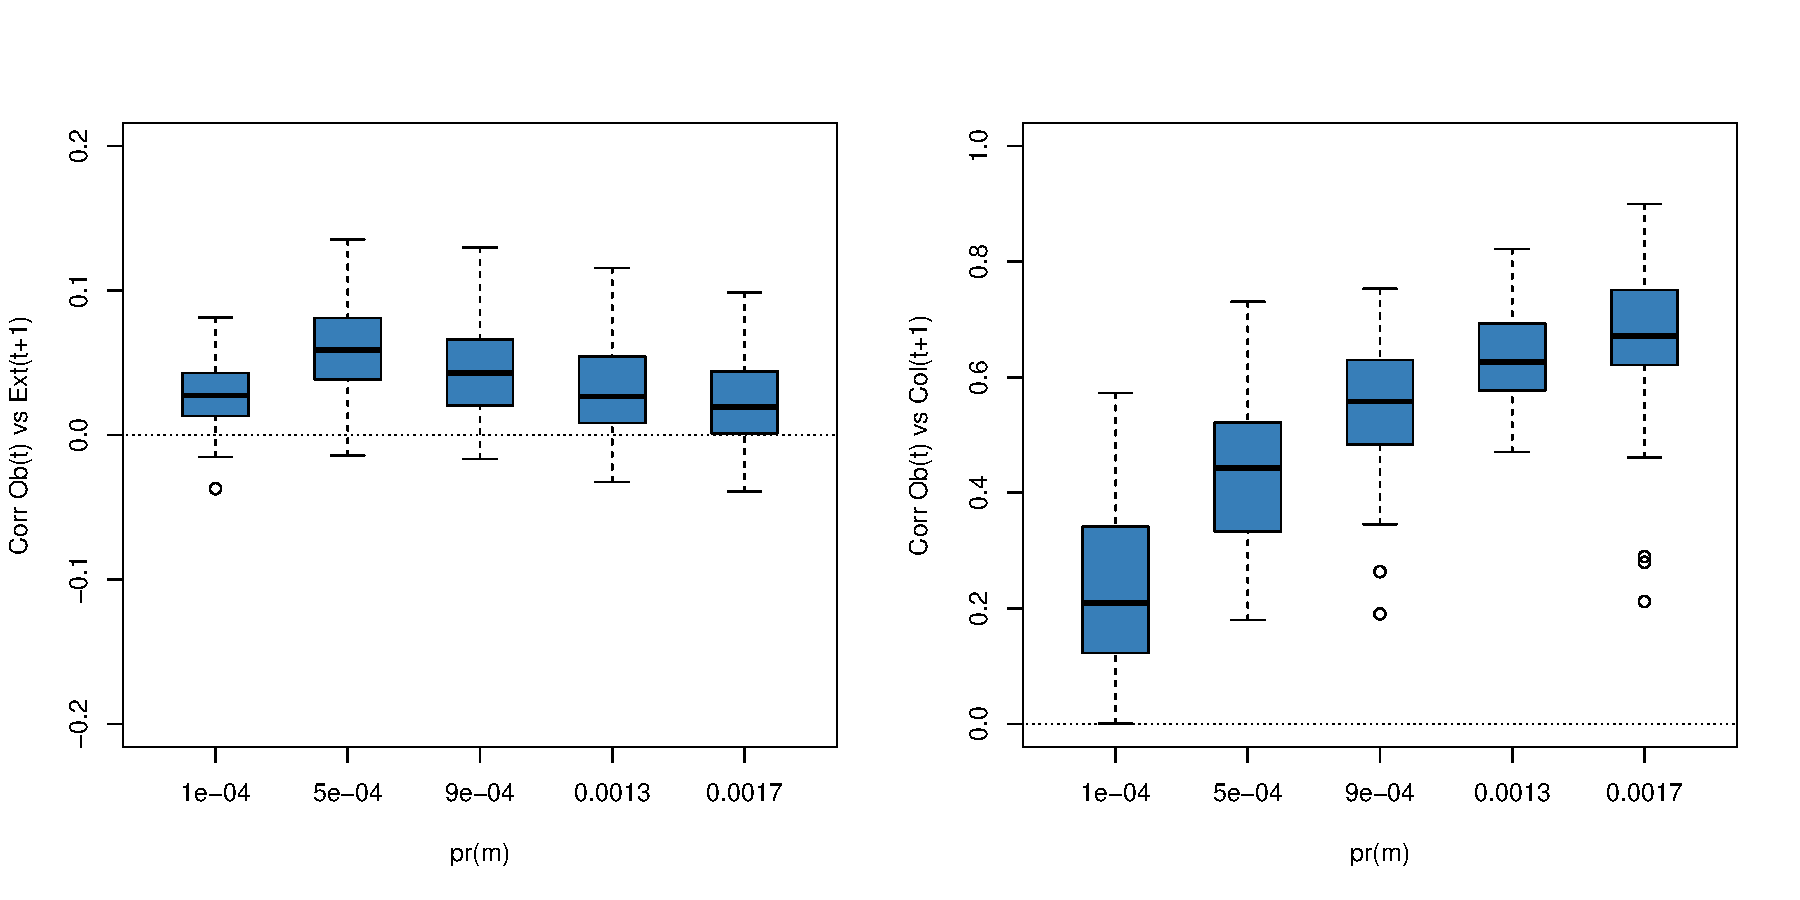
\includegraphics[width=0.75\textwidth]{fig_corrobext_tl2S.pdf}
% % \caption{
% % a) Correlations between objects at time $t$ and extinction cascade size at time $t+1$. b) Correlations between objects at time $t$ and the number of potential colonizers at time $t+1$.
% % }
% % \label{fig_corrobext}
% % \end{figure*} 
% 
% 
% Future things that I'm working on implementing (suggestions welcome!!!)
% \begin{enumerate}
% \item Calculate trophic level for each species
% \item Object decay - this is a big feature of engineered systems - that the objects they engineer can last longer than the species
% \item One potentially fruitful line of investigation would be to link this approach to random matrix theory - inclusion of objects should modify species effects on one another. I'm currently tracking both direct trophic and mutualistic adjacency matrices (where if species 1 makes object 1, and species 2 eats object 1, we can say species 2 indirectly eats species 1 - same for any other interaction type), but have not yet explored it - this would probably be good for a stand-alone paper - very little of engineering in food webs
% \item Priority effects - working on this - what species traits alter assembly dynamics?
% \end{enumerate}
% 


\end{document}
